\documentclass{article}
\usepackage{tikz}
\usetikzlibrary{decorations.pathreplacing} % nécessaire pour les accolades

\begin{document}
	
	\begin{center}
		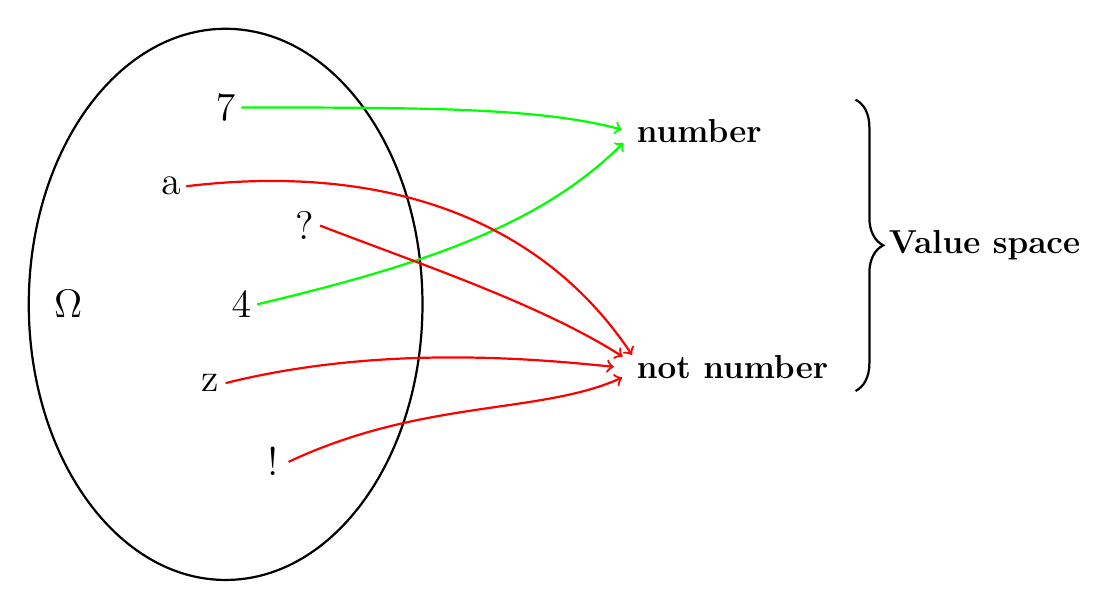
\begin{tikzpicture}[scale=1]
			
			% Ellipse à gauche
			\draw[thick] (-4,0) ellipse (2.5 and 3.5);
			
			% Nom de l'ellipse en majuscule
			\node at (-6,0) {\Large $\Omega$};
			
			% Caractères dans l'ellipse (plus gros)
			\node at (-4.0,2.5) {\Large 7};      % chiffre
			\node at (-4.7,1.5) {\Large a};      % lettre
			\node at (-3.0,1) {\Large ?};        % ponctuation
			\node at (-3.8,0) {\Large 4};        % chiffre
			\node at (-4.2,-1) {\Large z};       % lettre
			\node at (-3.4,-2) {\Large !};       % ponctuation
			
			% Labels à droite, verticalement espacés
			\node[right] (num) at (1.1,2.2) {\large \textbf{number}};
			\node[right] (notnum) at (1.1,-0.8) {\large \textbf{not number}};
			
			% Flèches vertes vers number
			\draw[->, thick, shorten >=2pt, green] (-3.8,2.5) .. controls (-1.5,2.5) and (0,2.5) .. (1.1,2.2);  % 7 -> number
			\draw[->, thick, shorten >=2pt, green] (-3.6,0)   .. controls (-1.5,0.5) and (0,1) .. (1.1,2.1);    % 4 -> number
			
			% Flèches rouges vers not number
			\draw[->, thick, shorten >=2pt, red] (-4.5,1.5) .. controls (-2,1.8) and (0,1.1) .. (1.2,-0.7);    % a -> not number
			\draw[->, thick, shorten >=2pt, red] (-4.0,-1) .. controls (-2,-0.5) and (0,-0.7) .. (1.0,-0.8);  % z -> not number
			
			\draw[->, thick, shorten >=2pt, red] (-2.8,1)   .. controls (-1.5,0.5) and (0,0) .. (1.1,-0.7);    % ? -> not number
			\draw[->, thick, shorten >=2pt, red] (-3.2,-2)  .. controls (-1.5,-1.2) and (0,-1.4) .. (1.1,-0.9);  % ! -> not number
			
			% Accolade à droite
			\draw[thick,decorate,decoration={brace,amplitude=10pt}] (4,2.6) -- (4,-1.1);
			
			% Texte à droite de l'accolade
			\node[right] at (4.3,0.75) {\large \textbf{Value space}};
			
		\end{tikzpicture}
	\end{center}
	
\end{document}
